\chapter{Analysis of Retract Force Curves in Colloidal Systems}

\section{Introduction}

\subsubsection{Analysis of Silica-silica retract curves}

In AFM, the study of force curves between silica surfaces in saline environments is a well explored avenue. However, the journey back from the surface — the retrace curve is often overlooked. Standard practice in AFM analysis tends to focus on the approach curves specifically, yet with every approach curve recorded, a corresponding retrace is inherently generated. However, a review of the literature reveals a conspicuous absence of retrace curve analysis; most studies emphasize the approach while relegating the retrace to a footnote, if it is acknowledged at all \cite{Retrace}. % \cite{John}.

This omission is understandable. Retrace curves can present a messier dataset, with the variability and complexity that derives from the chaotic nature of interactions when a tip withdraws from contact. This is due to a multitude of factors influencing the tip upon retraction: capillary forces, adhesion hysteresis, and tip contamination are but a few of the phenomena that can alter the tip's path back from the surface. While an approach curve starts from a place free of influence from the target in a stable part of a DLVO curve, the retrace starts at the point where it often is most complex.

Furthermore, DLVO theory, while capable in describing forces during the approach, can encounter hurdles when applied to the retrace curve. The symmetry of interaction predicted by DLVO when a tip approaches and retracts from a surface is often disrupted in practice. The retrace curve does not simply mirror the approach; it is influenced by history-dependent effects and irreversible changes to the tip or surface.

Within this chapter, we focus on these retrace curves, unpacking the generally noisier data in order to uncover the forces present between silica surfaces at the nanoscale. It is here where the complex analysis software shines, allowing conclusions to be drawn from curves that would otherwise be rejected.

The chapter advocates for a more holistic view in the field of AFM study, demonstrating that the insights gleaned from retrace curves are indispensable. considering both the approach and retraction events, a more complete picture of the interaction forces at play can be derived. The retrace curve, often overlooked, may hold the key to a deeper understanding of surface interactions, and it is time we turn our attention to this pivotal part of the AFM narrative.

The retraction phase often reveals information about the adhesive properties of the surface that might be masked or indistinguishable in the approach phase. Conversely, the approach phase is better suited to analyzing the initial contact mechanics without the confounding influence of adhesion. By analyzing these phases separately, we can study complex interactions between the tip and the sample surface within the context of the retaining adhesion. This separation allows for a more focused understanding of how the sample behaves under different mechanical conditions. \cite{BUTT20051}

\section{MFP-1D contact force derivation}

This section will overview the results for the following LiCl concentrations: 0.6mM, 1.6mM, 5mM, 10mM, 25mM, 50mM, 230mM, 550mM. For each concentration multiple sites are analysed, highlighting features of each curve in preparation for analysis. The analytical approach to processing this large dataset is given in Chapter 4. 

The removal of retract curves followed the same rationale as in the previous chapter, with these curves often overlapping with those removed during the approach phase. This overlap was primarily due to machine errors, such as unsuccessful surface contact or insufficient data points within the measurement window. Despite these necessary exclusions, the large volume of collected data ensured that the overall analysis remained robust and unaffected by the removals.

The graphs presented here have been carefully chosen from a large dataset to demonstrate key trends, ensure accurate representation of the interactions, and highlight the most significant features, such as the variability in the force profiles. While the strength of this work lies in the extensive dataset, selecting specific graphs allows for a more focused analysis of the most relevant data points.

The data processing involved analyzing thousands of individual curves, a process that comes with challenges, particularly due to the inherent noise and the influence of factors like capillary forces, adhesion hysteresis, or contamination during tip retraction. Ensuring a precise fit during the retract phase is crucial, as inaccuracies could lead to misleading interpretations.

Three types of graphs were selected to represent the behavior across different concentrations. The retract curves, constructed from binned averages, offer insights into the forces encountered during retraction. These curves are typically noisier in regions of adhesion, reflecting the variability in attractive forces.

The force versus Z-piezo position graph illustrates the forces as the tip disengages from the surface, highlighting the contact phase and helping to determine key interaction points. Lastly, the force histogram provides a clear visual of the distribution and variability of forces encountered during retraction, ensuring that the most probable interactions are accurately represented.

Each retrace corresponds to the same site defined in chapter 5, as this is the backward motion 

\insertretractfigures{6}{0.6}{1}{The retract curves generally show lower adhesion forces compared to higher ionic strengths. The curves reveal a weak attraction upon retraction, which is characteristic of low salt concentrations where van der Waals forces start to influence the interaction but are still relatively weak.

32 curves in total were processed. Of these processed curves the average attractive force was -0.3 nN $\pm$ 0.5 nN}
\insertretractfigures{6}{0.6}{2}{Site 2's retract data similarly exhibit weak adhesion, consistent with the approach data. However, the noise levels in the retract data are higher, which may obscure some finer details of the force interactions.

23 curves in total were processed. Of these processed curves the average attractive force was -0.04 nN $\pm$ 0.1 nN}
\insertretractfigures{6}{0.6}{3}{The retract curves at Site 3 show a similar trend, with weak adhesion forces and higher noise, reflecting the challenges of accurately measuring forces at low ionic strength.

29 curves in total were processed. Of these processed curves the average attractive force was -0.1 nN $\pm$ 0.2 nN}

0.6mM demonstrates the variability present in retrace curves. Occasionally, a retrace will have a higher attractive force. In general however, 0.6mM has very little to no attractive forces between the interacting elements.

%1.6
\insertretractfigures{6}{1.6}{1}{The retract curves for Site 1 show the expected behavior, with a slight increase in attractive forces as the AFM tip retracts from the surface. The retract curve’s widening in the attractive force region reflects the expected minor adhesive interactions that start to become more noticeable as ionic strength increases.

137 curves in total were processed. Of these processed curves the average attractive force was -0.1 nN $\pm$ 0.1 nN}
\insertretractfigures{6}{1.6}{2}{Similar to the approach curves, the retract curves for Site 2 continue to show complex interactions. The shelf behavior seen in the approach is also mirrored here, with a more pronounced widening in the retract phase, indicating persistent adhesion possibly due to the same surface irregularities or ion aggregates noted in Chapter 5.

112 curves in total were processed. Of these processed curves the average attractive force was -0.1 nN $\pm$ 0.2 nN}

1.6 mM has the same interesting shelf feature seen in the previous chapter. Interestingly - this shelf is largely in the same force range as the approach. Otherwise, 1.6 mM again has little attractive force, though notably more than 0.6mM.

%5
\insertretractfigures{6}{5}{1}{The retract curve shows a noticeable adhesive interaction, where the AFM tip experiences a clear pull-off force before fully disengaging from the surface. This is a significant change from the behavior seen at lower concentrations, indicating that the balance between repulsive and attractive forces is shifting as ionic strength increases.
The contact region of this graph also demonstrates a bend in the data. This can sometimes occur in the data, where theory meets reality. In this case it could be where the cantilever is bending non linearly during the contact phase, or where the surface hardness may be variable. It may also arise from surface roughness or surface indentations.

128 curves in total were processed. Of these processed curves the average attractive force was -0.8 nN $\pm$ 0.9 nN}
\insertretractfigures{6}{5}{2}{In comparison to site 1, the attractive force is less dramatic, missing the adhesion event seen before.
The contact region demonstrates a slight drift in the data. In this case it is likely from a slightly imperfect fit. In this case the fit is adequate to use however as the deviation from adjusting to the other direction does not impact the contact force significantly. Additionally, in some cases, a perfect fit cannot be reached from how the script is set up to process the data, or the average between all of the curves causes a tilt by how the script attempts to fit across the dataset range.

99 curves in total were processed. Of these processed curves the average attractive force was -0.1 nN $\pm$ 0.2 nN}
\insertretractfigures{6}{5}{3}{The retract curve at this site is comparable to Site 2, showing a weaker adhesive interaction. The curve seen in the contact phase is likely due cantilever non-uniformity or drift during measurement or surface roughness.

113 curves in total were processed. Of these processed curves the average attractive force was -0.1 nN $\pm$ 0.2 nN}

At the concentration of 5 mM LiCl, the range of pull-off forces shows increased variability, which is reflected in the binned points of the average curve after fitting. This variability arises from differences in the distances at which the cantilever "jumps out" from adhesive contact with the surface. The observed curvature in the contact area may indicate drift during the contact phase, potentially exacerbated by prolonged contact time between the tip and the surface. Furthermore, the characteristic "shelf" feature is clearly visible at all three sites, consistent with the observations from the approach curves.

%10 2 sites
\insertretractfigures{6}{10}{1}{The force at contact shows a distinct negative deflection indicative of an adhesive interaction. This suggests that at this concentration, the ionic environment supports a stable but weak adhesive interaction between the tip and the silica surface, which is quickly overcome as the tip retracts. The range of forces is also more significant, with some retractions containing a significant attractive force.

130 curves in total were processed. Of these processed curves the average attractive force was -0.6 nN $\pm$ 1.1 nN}
\insertretractfigures{6}{10}{2}{The retract curve at Site 2 for 10mM LiCl also exhibits a similar adhesive interaction at the point of contact, with a force profile that closely matches that of Site 1. However the presence of the shelf is observed in the data, and range of forces is reduced.

119 curves in total were processed. Of these processed curves the average attractive force was -0.2 nN $\pm$ 0.1 nN}
\insertretractfigures{6}{10}{3}{Site 3 demonstrates a curve similar to site 2, with a shelf feature and a weakly attractive surface.

123 curves in total were processed. Of these processed curves the average attractive force was -0.1 nN $\pm$ 0.1 nN}

10mM starts to transition from a the occasional adhesive retrace curve, to a distribution of attractive ranges. The attractive forces measured at sites 2 and 3 are distributed in a manner more similar to a normal distribution than those measured at site 1. Site 1 has a greater ranges of forces observed, possibly indicating a unique surface topology or potentially interaction of contaminants and is the only site in this group to not have the shelf feature present.

%25 3 sites
\insertretractfigures{6}{25}{1}{Site 1 presents a strong attractive force with a wide range of attractive forces. Additionally, the shelf feature can be seen in the data. This is a dramatic increase in the observed attractive force from the previous concentration. The disengage profile is much wider, indicating that the tip may be caught up in something, possibly due to contamination.

145 curves in total were processed. Of these processed curves the average attractive force was -2.2 nN $\pm$ 1.4 nN}
\insertretractfigures{6}{25}{2}{Site two still presents a significant attractive force, with the presence of the shelf seen in the data. However, the force recorded is almost half of site one, with a much smaller force range observed. The disengage profile seen is more similar to what would be expected with a a single disengage event, and in line with the other events seen in the dataset.

124 curves in total were processed. Of these processed curves the average attractive force was -0.8 nN $\pm$ 0.2 nN}
\insertretractfigures{6}{25}{3}{Site three presents a curve more similar to site 1, with a shelf, wider range of measured forces, a wide and noisy disengage profile and a strong attraction. The observed shelf also is unusual in that the jump from contact is more of a linear approach to contact, which arises from the range at which the tip disengages the surface.

92 curves in total were processed. Of these processed curves the average attractive force was -4.2 nN $\pm$ 2.0 nN}

25 mM presents an unusual collection of data, largely due to the high range of forces observed. It also presents a significant increase in the observed forces, and also a noisy disengage in 2 of the 3 sites. Site 3 also has an unusual looking shelf with respect to the rest of the observed shelves in the dataset, and is due to the noise in the data, as individual curves display a snap from contact as expected. The range of forces, both in terms of the range observed and the average across the dataset is unusual, as this marks a dramatic increase in the variability between sites and the force observed. This coupled with the disengage profile being unusual indicates that the 25 mM solution may have been contaminated during the procedure.

%50 2 sites
\insertretractfigures{6}{50}{1}{Site 1 demonstrates a return to previously seen values, following the trend of a slight attractive force observed between the surface and the tip. The shelf feature is also here, with a observed snap to contact.

104 curves in total were processed. Of these processed curves the average attractive force was -0.2 nN $\pm$ 0.1 nN}
\insertretractfigures{6}{50}{2}{Site 2 provides a similar curve to site 1, with a different in the shelfs snap from contact. This is due to the data in this site having a range in which the jump from contact occurs, thus flattening out the curve.

105 curves in total were processed. Of these processed curves the average attractive force was -0.2 nN $\pm$ 0.05 nN}

50 mM curves show a return to form defined by the other concentrations, outside of 25 mM. A slightly attractive force with a shelf feature. The attractive force is roughly in line with the other observed concentrations. The red dots seen on the curve indicate the data points used to align contact region.

%230 2 sites
\insertretractfigures{6}{230}{1}{Site 1 shows a significant increase of attractive force between the tip and the surface. This is likely due to the salt ions screening the electrostatic repulsion to a significant degree, allowing the attractive forces to dominate for longer. 

105 curves in total were processed. Of these processed curves the average attractive force was -1.2 nN $\pm$ 0.5 nN}
\insertretractfigures{6}{230}{2}{Site 2 presents a similar curve to site 1, with a significant attractive force of around 1 nN. Both sites present an expected disengage profile.

103 curves in total were processed. Of these processed curves the average attractive force was -0.9 nN $\pm$ 0.2 nN}

230mM marks a shift in the dataset so far; a significant increase of attractive force, with coherent force curves with this change. As such, unlike 25 mM, this change in attractive force is supported by two force curves reporting similar effects and is more robust. This shift is likely due to the balance of force shifting away from electrostatic repulsion, as the screening effect reduces it's impact.

%550 3 sites
\insertretractfigures{6}{550}{1}{Site 1 shows an increase of attractive force, with a coherent disengage profile and noise profile. The shelf feature is clearly present, with a jump from contact observed.

117 curves in total were processed. Of these processed curves the average attractive force was -1.7 nN $\pm$ 0.3 nN}
\insertretractfigures{6}{550}{2}{Site 2 demonstrates a similar curve to site 1, with an overall lower observed attractive force. The contact region of the curve for this site was particularly difficult to fit, either due to drift of potentially the interacting surface roughness. This site also has the shelf feature.

96 curves in total were processed. Of these processed curves the average attractive force was -0.7 nN $\pm$ 0.2 nN}
\insertretractfigures{6}{550}{3}{Site 3 shows a slight deviation from the other two sites, in that the shelf feature is not present in the curve. Otherwise the disengage profile is coherent, and the attractive force measured is similar to the other sites, adding evidence that the shelf feature's presence may not impact the measured force at contact.

112 curves in total were processed. Of these processed curves the average attractive force was -1.5 nN $\pm$ 0.2 nN}

The final concentration follows the trend that 230mM shows, a marked increase of attractive force. Across the 3 sites observed the data collected agrees with each other, and appears coherent.

\section{Overall force vs LiCl concentration graphs}

The pull off forces calculated were subsequently averaged, with the standard deviation calculated using equation \ref{eq:Stdevavg}.

\begin{figure}
    \centering
    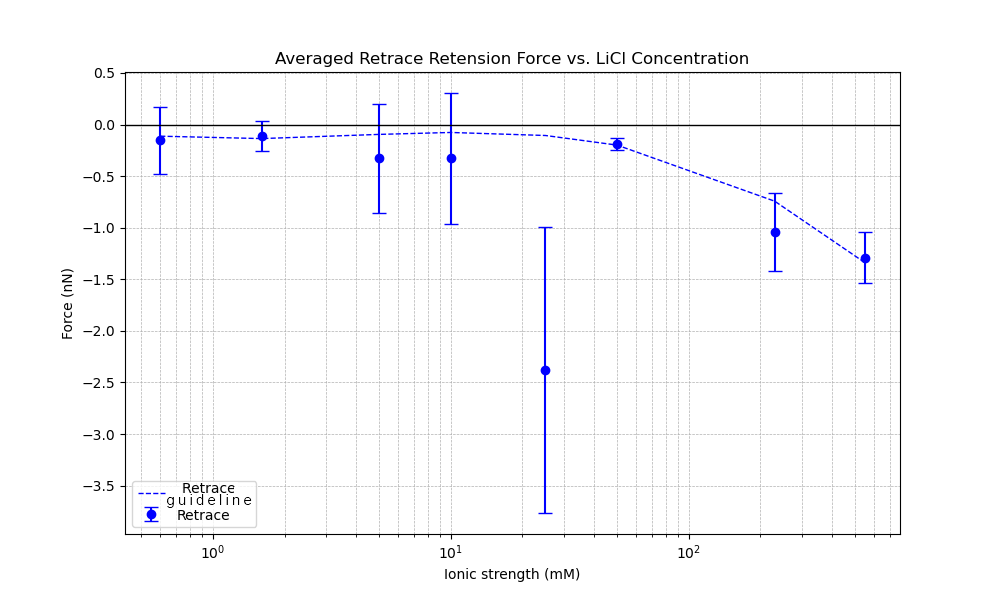
\includegraphics[width=1\linewidth]{chapter6/Averages.png}
    \caption{Site one calculated attraction force from contact with standard deviation error bars.}
    \label{fig:site1cont}
\end{figure}


The retrace curve shown in figure \ref{fig:site1cont} represents the attractive forces that are retained when the AFM tip is retracted from the contact with the surface at different LiCl concentrations. The retraction curve exhibits a plateau in attractive force up to a critical concentration of approximately 50mM, after which the attractive force between the AFM tip and the surface intensifies with increasing LiCl concentration. However 25mM is perplexing, as it demonstrates the strongest attractive force, though it is worth noting that 25mM was also a bit of an oddity in the approach curves due to it's higher standard deviation. This could be due to other reasons, such as a unexpected surface perturbation providing additional friction. In general, however, there is a trend of increasing attractive force past 50mM concentration, and thus pull off force across the datapoints.

Another aspect that stands out is the prominence of the standard deviation, especially at the higher concentrations. This is typical for retrace curves due to the reasons mentioned earlier such as tip changes upon contact. It is also interesting to note that the attractive forces in retrace curves are usually not symmetrical with the approach curves due to various interactions that can occur when the tip is in contact with the surface. These interactions include adhesion hysteresis, capillary forces, and possible tip contamination or wear, which can all affect the tip as it retracts and lead to the variability observed.

To better understand the behavior observed at higher salt concentrations, a comparison with DLVO theory serves as a foundational starting point. According to DLVO predictions, the balance between electrostatic repulsion and van der Waals attraction should govern the force profiles observed. As ion concentration increases, this attraction should decrease. 

This is somewhat reflected in the data, towards the end of the dataset, from 50 mM to 550 mM. One significant outlier is 230 mM however, as this demonstrates a significant deviation from the observed trend and is highly suspect. Given that 25 mM has a high degree of variability in the observed data, and has unique features in the collected data, it may be that the 25 mM solution itself was contaminated, or the tip used for this data set was unsuitable. The significant disengage profile observed in this dataset, coupled with the high degree of noise, also provides credibility to this consideration.

One key factor that can contribute to the trends observed in the retract curves, particularly at higher LiCl concentrations, is surface roughness. As indicated by Bhattacharjee et al. (1998) \cite{Bhattacharjee1998}, surface roughness can significantly reduce the repulsive forces predicted by classical DLVO theory, especially when the roughness scale is comparable to the Debye length. This reduction in repulsion could lead to stronger net attractive forces at higher salt concentrations, as observed in the 50 mM to 550 mM range. The reduction in repulsive barriers allows the attractive van der Waals forces to become more prominent, which is consistent with the increasing pull-off forces seen in the data.

Additionally, the concept of charge regulation might further explain the behavior at these higher concentrations. As discussed by Guleryuz et al. (2012) \cite{Guleryuz2012}, at higher ionic strengths, the surface charge density can change due to the changing ionic environment. This charge regulation could lead to a more uniform distribution of charges across the surface, thereby enhancing the attractive interactions between the AFM tip and the silica surface. This adjustment could result in the more consistent attractive forces observed beyond the 50 mM concentration, where the repulsive forces become less dominant. Zhao et al. (2015) \cite{zhao2015} discusses how surface charge at solid-electrolyte interfaces is influenced by the adsorption and desorption of ions, which directly affects the electrostatic potential near the surface. This could imply that the increase in attractive force at concentrations above 50 mM could be due to enhanced ion adsorption at the interface. \cite{Afekare2020}

Moreover, the presence of a 'shelf' in the force profiles suggests the involvement of additional forces or mechanisms not fully captured by DLVO theory. The shelf could indicate the formation of structured hydration or solvation layers on the silica surface, as discussed by Kostakis et al. (2006) \cite{Kostakis2006}. These layers could introduce an additional attractive component or a barrier that modifies the interaction profile during the retraction phase. This phenomenon may explain why the forces do not decrease smoothly with increasing salt concentration, but instead show complex behavior that varies across different sites. This shelf feature is looked into more detail in Chapter 8.

One final interesting note is the observation of the 50mM tipping point present in both the approach and retrace curve, indicating that past 50mM there potentially could be some kind of mechanism that impacts the electrostatic repulsion, rather than a build up of ions on the surface. I.e. the gradual accumulation of ions that might lead to a saturated surface charge density. This process is akin to charge regulation, where the surface charge adjusts in response to the ionic strength of the surrounding solution. At higher concentrations, this regulation could lead to a more uniform distribution of forces, as observed in the force profiles. This could mean that for surfaces in contact DLVO may behave differently and the interacting surface area could be added to DLVO to model how surfaces already in contact have a reduced area for ions to screen charge. Beyond this tipping point, the surface may become saturated with ions, leading to a stabilization of the electrostatic environment and a corresponding increase in attractive forces. This hypothesis aligns with the broader understanding of how surface charge density and ionic strength interact to influence colloidal stability and interfacial forces. \cite{israelachvili2011intermolecular}

Given the observed complexities, an extended DLVO framework is may be required to fully capture the nuances of the interfacial forces at play, particularly at higher ionic strengths. One potential extension could involve the incorporation of a dynamic charge regulation model, which would account for the real-time adjustments of surface charge in response to the local ionic environment. This would involve not only considering the magnitude of the surface charge but also how it evolves as ions adsorb or desorb from the surface, potentially leading to time-dependent changes in the force profiles observed.

Furthermore, the inclusion of surface roughness effects could provide a more accurate prediction of force behaviors in systems where the physical characteristics of the surface play a significant role. Another possible extension could be the incorporation of hydration or solvation layers to influence the interaction profiles significantly. These layers could introduce short-range forces that modify the expected DLVO interactions, particularly in the presence of high salt concentrations where the classical assumptions of the theory may no longer hold.

In the following chapter, we will explore these concepts further and discuss their implications for the theoretical modeling of interfacial forces.